\chapter{动物如何繁殖}\label{ch:g4:animal-reproduction}

五月，池塘里蛙声阵阵；到了六月，池塘已被
\omterm{ex:g2:animals-grow-up:frog}{蝌蚪}染得一片漆黑。原来，那阵蛙鸣正是这个故事的开端：
繁殖——\omterm{def:g1:animals-around-us:animal}{动物}如何产生下一代——
遵循着从青蛙到大象都适用的规律，
只是细节上千变万化。

\section{需要两个亲本}

\begin{definition}[有性生殖]\label{def:g4:animal-reproduction:sexual}
在\omterm{def:g1:animals-around-us:animal}{动物}中，繁殖后代通常需要两个亲本：一个
\emph{雌性}\index{雌性}和一个\emph{雄性}\index{雄性}。
雌性产生\emph{卵细胞}\index{卵细胞}；雄性
产生\emph{精子}\index{精子}。一个幼体始于一个精子与一个
卵细胞结合，这种结合
称为\emph{受精}\index{受精}。由两位亲本完成的
繁殖，叫作
\emph{有性生殖}\index{有性生殖}。
\end{definition}

\begin{example}[青蛙为何鸣叫]\label{ex:g4:animal-reproduction:song}
五月的合唱，是雄蛙把雌蛙
召至池塘。随后，每对蛙把各自的
细胞排入水中——雌蛙的卵，雄蛙的
\omterm{def:g4:animal-reproduction:sexual}{精子}——\omterm{def:g4:animal-reproduction:sexual}{受精}就在这里发生。几天后
果冻团里的黑点，已是正在生长的幼体；鸣唱正是
\cref{ch:g2:animals-grow-up}中青蛙循环的第一步。
\end{example}

\begin{omfigure}
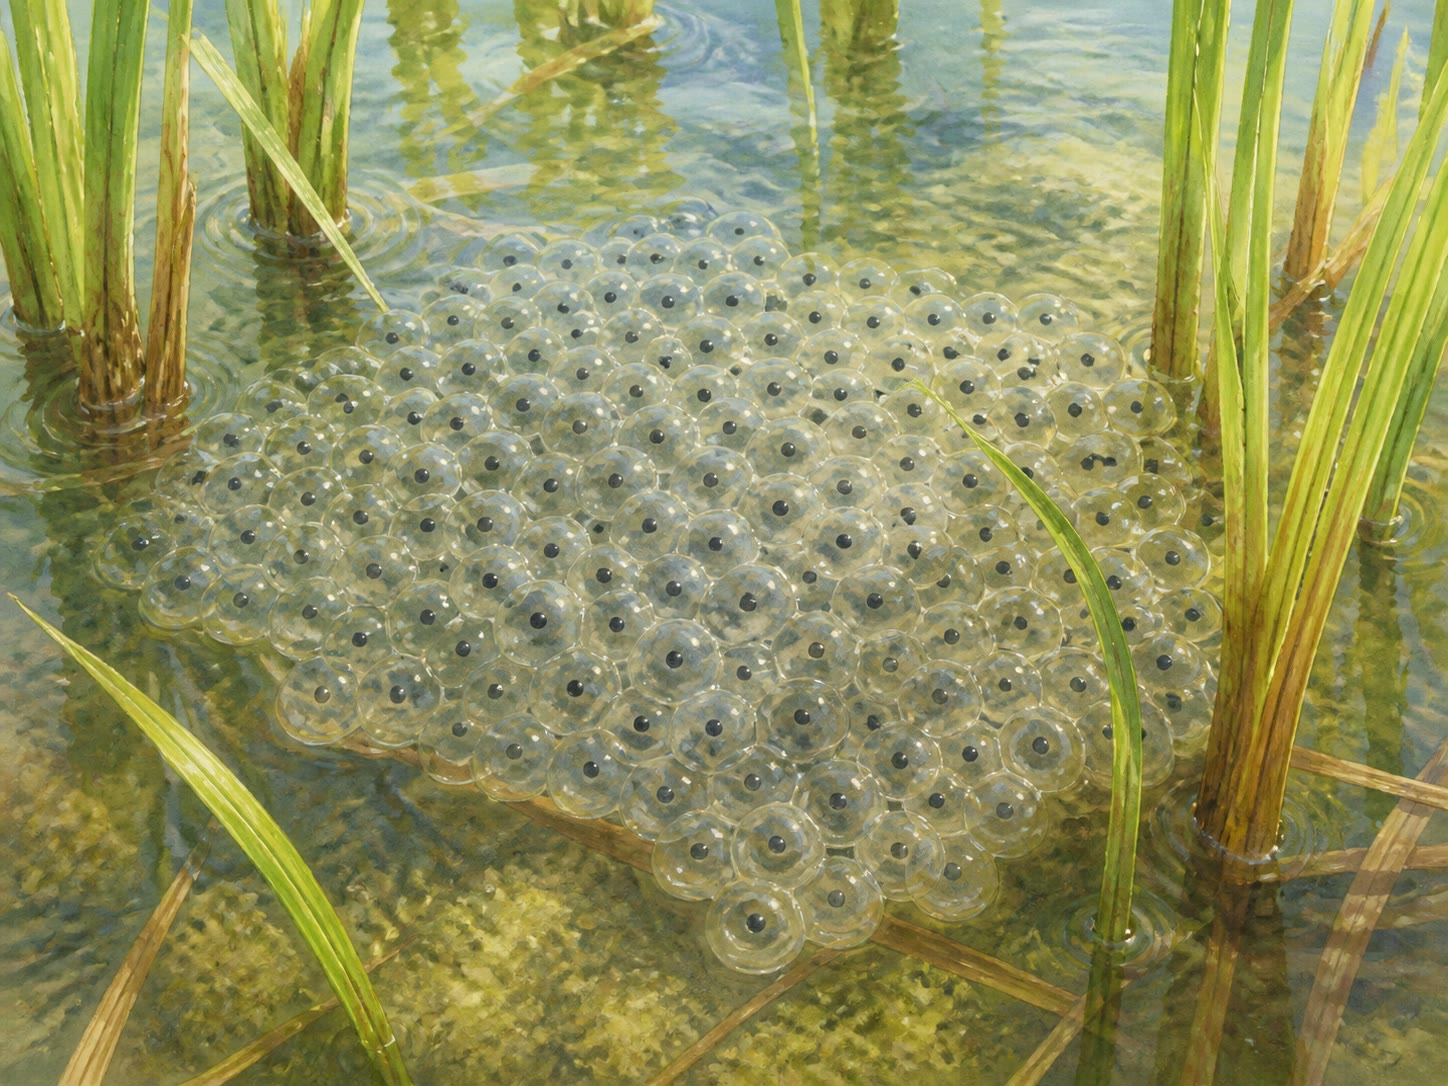
\includegraphics[width=0.56\linewidth]{images/book1/ai/g4-repro-frogspawn.jpg}

{\small 合唱几天后：芦苇间的蛙卵团，
每个果冻球都是一枚\omterm{def:g4:animal-reproduction:sexual}{受精}卵，里面
已开始孕育小蛙。}
\end{omfigure}

\begin{remark}[双亲，混合的运气]\label{rem:g4:animal-reproduction:mix}
幼体从每个亲本那里各获得一些东西——这正是小马
能同时拥有母马毛色与父马白色额斑的原因。
每个亲本究竟传递什么、如何传递，是本书
后面要探讨的重大问题之一；现在只需记住，
每个有性产生的\omterm{def:g1:animals-around-us:animal}{动物}都有两个亲本，
并且同时与双亲相似。
\end{remark}

\section{产卵，还是胎生}

\begin{definition}[卵生与胎生]\label{def:g4:animal-reproduction:ovivivi}
\Cref{def:g2:animals-grow-up:born}中的两种出生方式，
现在有了各自的学名：
\begin{itemize}
  \item \omterm{def:g1:animals-around-us:animal}{动物}为\emph{卵生}\index{卵生}，是指
        \omterm{def:g4:animal-reproduction:sexual}{雌性}产\emph{卵}，幼体在卵内、母体之外完成发育：
        \omterm{prop:g3:sorting-living-things:groups}{鸟类}、大多数\omterm{prop:g3:sorting-living-things:groups}{鱼类}、
        大多数\omterm{prop:g4:classifying-animals:classes}{爬行动物}、\omterm{prop:g3:sorting-living-things:groups}{两栖动物}、\omterm{prop:g3:sorting-living-things:groups}{昆虫}、蜗牛；
  \item \omterm{def:g1:animals-around-us:animal}{动物}为\emph{胎生}\index{胎生}，是指
        幼体在\emph{母体内}生长，由母体供养，
        并\emph{\omterm{def:g2:animals-grow-up:born}{胎生出生}}：几乎所有\omterm{prop:g3:sorting-living-things:groups}{哺乳动物}。
\end{itemize}
\end{definition}

\begin{example}[两种育幼方式]\label{ex:g4:animal-reproduction:nurseries}
母鸡的雏鸟在有壳的卵中
度过三个温暖的星期，靠卵黄维持生长（\cref{rem:g2:animals-grow-up:egg}）；
小马驹在母马体内度过十一个月，
由母体不断供养，出生后一小时内就能站立。
目标相同，育幼方式却不同：一种是壳中的
便当，一种是体内的送餐服务。
\end{example}

\begin{proposition}[受精发生的地点]\label{prop:g4:animal-reproduction:where}
对于\omterm{prop:g3:sorting-living-things:groups}{鱼类}和青蛙等水生\omterm{def:g1:animals-around-us:animal}{动物}，\omterm{def:g4:animal-reproduction:sexual}{受精}通常
发生在\emph{水中}，即\omterm{def:g4:animal-reproduction:sexual}{雌性}体外——卵和\omterm{def:g4:animal-reproduction:sexual}{精子}
同时排入水中相遇，数以千计。对于陆生\omterm{def:g1:animals-around-us:animal}{动物}——\omterm{prop:g3:sorting-living-things:groups}{鸟类}、\omterm{prop:g4:classifying-animals:classes}{爬行动物}、\omterm{prop:g3:sorting-living-things:groups}{哺乳动物}、\omterm{prop:g3:sorting-living-things:groups}{昆虫}——
细胞暴露在空气中会干燥失效，因此\omterm{def:g4:animal-reproduction:sexual}{雄性}
将\omterm{def:g4:animal-reproduction:sexual}{精子}送入\omterm{def:g4:animal-reproduction:sexual}{雌性}\emph{体内}，
即在\emph{交配}\index{交配}过程中完成，
\omterm{def:g4:animal-reproduction:sexual}{受精}便在那里发生。
\end{proposition}
\admitted

\section{幼体少而精心呵护，或多而不顾}

\begin{proposition}[延续后代的两种策略]\label{prop:g4:animal-reproduction:strategies}
比较一下数量：鳕鱼每年产下\emph{数百万}枚卵，
却一枚也不照料；大象仅有\emph{一}头幼崽，
每隔几年生一头，并守护它长达十年。在这两个极端之间，
\omterm{def:g1:animals-around-us:animal}{动物}界有一条规律：后代越多，每个后代得到的照料
就越少；后代越少，每个后代就越受保护、越能获得食物。
两种策略都能成功：平均而言，
总有足够的后代存活下来，
得以替代亲代。
\end{proposition}
\admitted

\begin{example}[数一数池塘]\label{ex:g4:animal-reproduction:pondcount}
一对青蛙产下的卵块含有数千枚卵。苍鹭、
刺鱼和蜻蜓幼虫（见\cref{ex:g3:food-chains:three}）
整个春天都在吞食\omterm{ex:g2:animals-grow-up:frog}{蝌蚪}——
在数千枚卵中，只有一小撮幼蛙能在七月
爬上岸边。庞大的卵块并非浪费，而是青蛙
应对池塘危险的办法，它们完全不需要亲代守护。
\end{example}

\begin{example}[另一个极端]\label{ex:g4:animal-reproduction:whalecalf}
鲸鱼幼崽独自出生，出生后立即在母亲身边游动，
吮吸母亲营养丰富的\omterm{def:g2:animals-grow-up:born}{乳汁}长达数月，并
免受各种危险的威胁。一次只生一个
幼体，但这个幼体获得了一切。\omterm{prop:g3:sorting-living-things:groups}{哺乳动物}凭借其
\omterm{def:g2:animals-grow-up:born}{乳汁}（\cref{def:g2:animals-grow-up:born}），
成为“少生、精心养育”策略的最佳代表。
\end{example}

\begin{method}[阅读一个物种的策略]\label{met:g4:animal-reproduction:read}
给定一个物种，提问：
\begin{enumerate}
  \item 一次生育几个幼体？一个、一打，还是数千个？
  \item 由谁守护和喂养它们——双亲、母亲，
        还是无人？
  \item 幼体在哪里开始发育——卵在体外，还是在体内发育？
  \item 核对
        \cref{prop:g4:animal-reproduction:strategies}中的权衡：
        是幼体多而少照顾，还是少而精心照顾。
\end{enumerate}
\end{method}

\section{练习}

\begin{exercise}[$\star$]\label{exo:g4:animal-reproduction:1}
什么是\omterm{def:g4:animal-reproduction:sexual}{受精}？每个亲本分别提供哪种细胞？
\end{exercise}

\begin{exercise}[$\star$]\label{exo:g4:animal-reproduction:2}
给出\omterm{def:g4:animal-reproduction:ovivivi}{卵生}与\omterm{def:g4:animal-reproduction:ovivivi}{胎生}的定义，每类各举
两种\omterm{def:g1:animals-around-us:animal}{动物}。
\end{exercise}

\begin{exercise}[$\star$]\label{exo:g4:animal-reproduction:3}
为什么青蛙在五月鸣叫？用三步复述
池塘里的故事。
\end{exercise}

\begin{exercise}[$\star$]\label{exo:g4:animal-reproduction:4}
鳟鱼的\omterm{def:g4:animal-reproduction:sexual}{受精}发生在哪里，
母鸡的\omterm{def:g4:animal-reproduction:sexual}{受精}在哪里？两者为何不同，依据
\cref{prop:g4:animal-reproduction:where}？
\end{exercise}

\begin{exercise}[$\star$]\label{exo:g4:animal-reproduction:5}
比较雏鸡与马驹的“育儿场所”：各自
在哪里生长，又由什么提供养分？
\end{exercise}

\begin{exercise}[$\star$]\label{exo:g4:animal-reproduction:6}
说出幼体数量与所获照顾之间的规律，
并举出本章的两个极端例子。
\end{exercise}

\begin{exercise}[$\star$]\label{exo:g4:animal-reproduction:7}
鳕鱼的数百万个卵大多永远长不成成年鳕鱼。
这种策略为何仍然成功？
\end{exercise}

\begin{exercise}[$\star$]\label{exo:g4:animal-reproduction:8}
对猫运用\cref{met:g4:animal-reproduction:read}：典型的
一窝约五只，由母亲哺育并守护
数周，在母体内发育。它更接近哪一种策略？
\end{exercise}

\begin{exercise}[$\star\star$]\label{exo:g4:animal-reproduction:9}
马驹常常同时像父母双方。这说明
幼体所获得的是什么，依据
\cref{rem:g4:animal-reproduction:mix}？
\end{exercise}

\begin{exercise}[$\star\star$]\label{exo:g4:animal-reproduction:10}
棘鱼雄鱼筑巢、扇动卵块，并
驱赶入侵者——对\omterm{prop:g3:sorting-living-things:groups}{鱼类}而言这种付出实属罕见。借助
\cref{prop:g4:animal-reproduction:strategies}，请推测
它一窝卵的数量与鳕鱼的数百万相比，
会有怎样的差异？
\end{exercise}

\begin{exercise}[$\star\star\star$]\label{exo:g4:animal-reproduction:11}
海龟爬上岸，把卵埋在温暖的沙中，然后
返回大海。属于\omterm{def:g4:animal-reproduction:ovivivi}{卵生}还是\omterm{def:g4:animal-reproduction:ovivivi}{胎生}？是否受到照顾？
这种\omterm{prop:g4:classifying-animals:classes}{爬行动物}一生都在水中游动，为何仍须
在\emph{陆地}上产卵？（运用\cref{prop:g4:classifying-animals:classes}中的
\omterm{prop:g4:classifying-animals:classes}{爬行动物}特征。）
\end{exercise}
